\section{Artigos}

Foi realizada uma pesquisa na plataforma \emph{Google Scholar} com o objetivo de identificar trabalhos correlatos desenvolvidos nos últimos cinco anos (2021 a 2025). Utilizaram-se as palavras-chave "Estrutura de Dados", "Jogo Sério" e "Desenvolvimento", o que resultou inicialmente em um total de 45 artigos.

Após uma análise preliminar, 40 artigos foram descartados por não envolverem o desenvolvimento de um jogo ou por tratarem de jogos cuja temática não estava relacionada à área de programação. Com isso, restaram 5 artigos para uma avaliação mais aprofundada.

Os artigos selecionados para essa etapa de análise detalhada foram aqueles que atenderam simultaneamente aos seguintes critérios: aplicação de jogo sério no ensino de programação e apresentação de um protótipo funcional ou em desenvolvimento. Sendo estes:

\begin{enumerate}
  \subsection{CodingJob: Um jogo sério para auxiliar nas disciplinas de Linguagem de Programação C}

Esta dissertação apresenta o jogo \textit{CodingJob}, um jogo sério que fornece um ambiente para prática dos conhecimentos da disciplina de \textit{Linguagem e Programação I} utilizando a linguagem C. \cite{costa2023condigjob}

\begin{figure}[H]
	\centering
	\caption{Captura de tela do jogo CodingJob}
	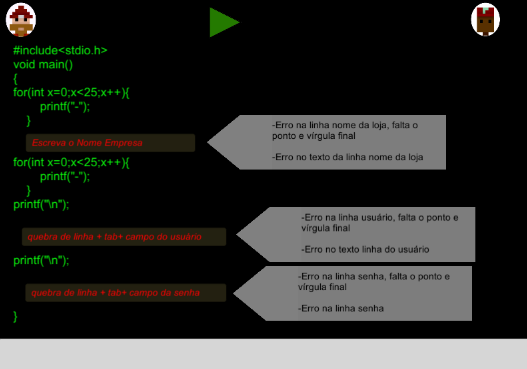
\includegraphics[width=0.8\textwidth]{images/codingjob.png}
	\legend{Fonte: \cite{costa2023condigjob}}
	\label{fig:codingjob}
\end{figure}



  \subsection{CodeBô: Design e avaliação de um puzzle game para o ensino de Estrutura de Dados}

O intuito do projeto \emph{CodeBô} foi desenvolver um jogo digital isométrico de \emph{puzzles} que se baseia na mecânica do \emph{lightBot}, um jogo mobile educacional conceituado, mecânica esta que consiste em selecionar uma ordem de movimentos que o personagem deve executar para se mover até um local específico. O jogo \emph{CodeBô} utiliza essas mecânicas para ensinar conceitos como Pensamento Computacional, pilhas, filas e listas. \cite{de2025codebo}

\begin{figure}[H]
	\centering
	\caption{Captura de tela do jogo CodeBô}
	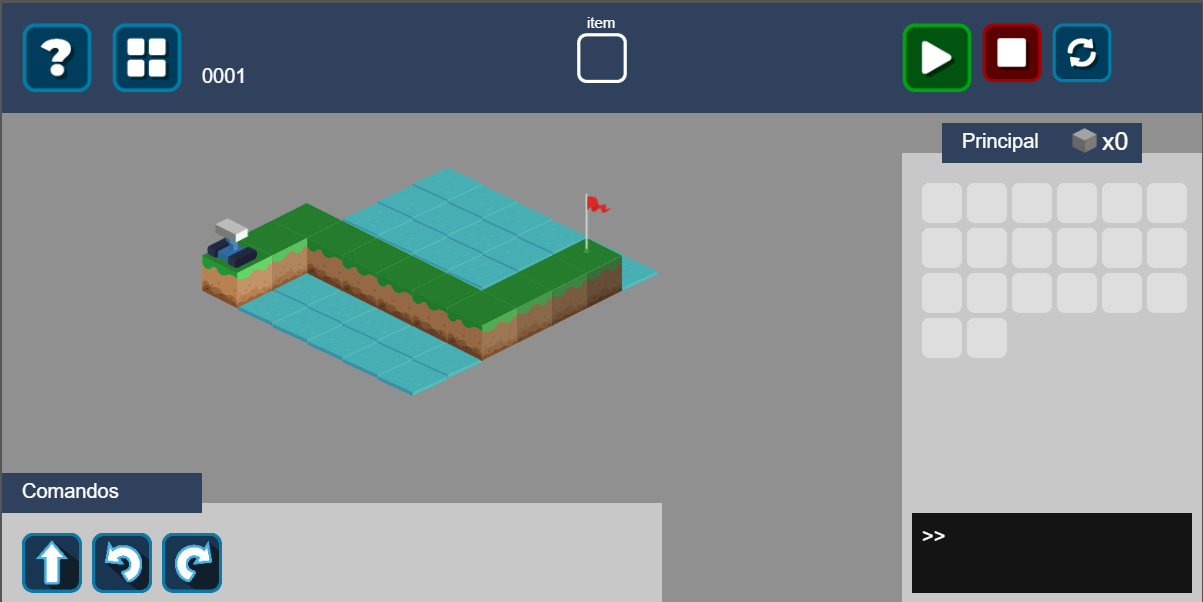
\includegraphics[width=0.8\textwidth]{images/codebo.png}
	\legend{Fonte: \cite{de2025codebo}}
	\label{fig:codebo}
\end{figure}



  \item \textbf{CodeBo Unplugged: Um jogo desplugado para o ensino de Pilha}

O jogo de tabuleiro CodeBo Unplugged \cite{de2023codebo} foi desenvolvido com o intuito de
ensinar a estrutura de dados Pilha a alunos do ensino fundamental de forma
lúdica, utilizando elementos como robôs e mapas que aumentam em dificuldade de
forma progressiva. \cite{de2023codebo}

\begin{figure}[H]
	\centering
	\caption{Foto do tabuleiro de CodeBô Unplugged}
	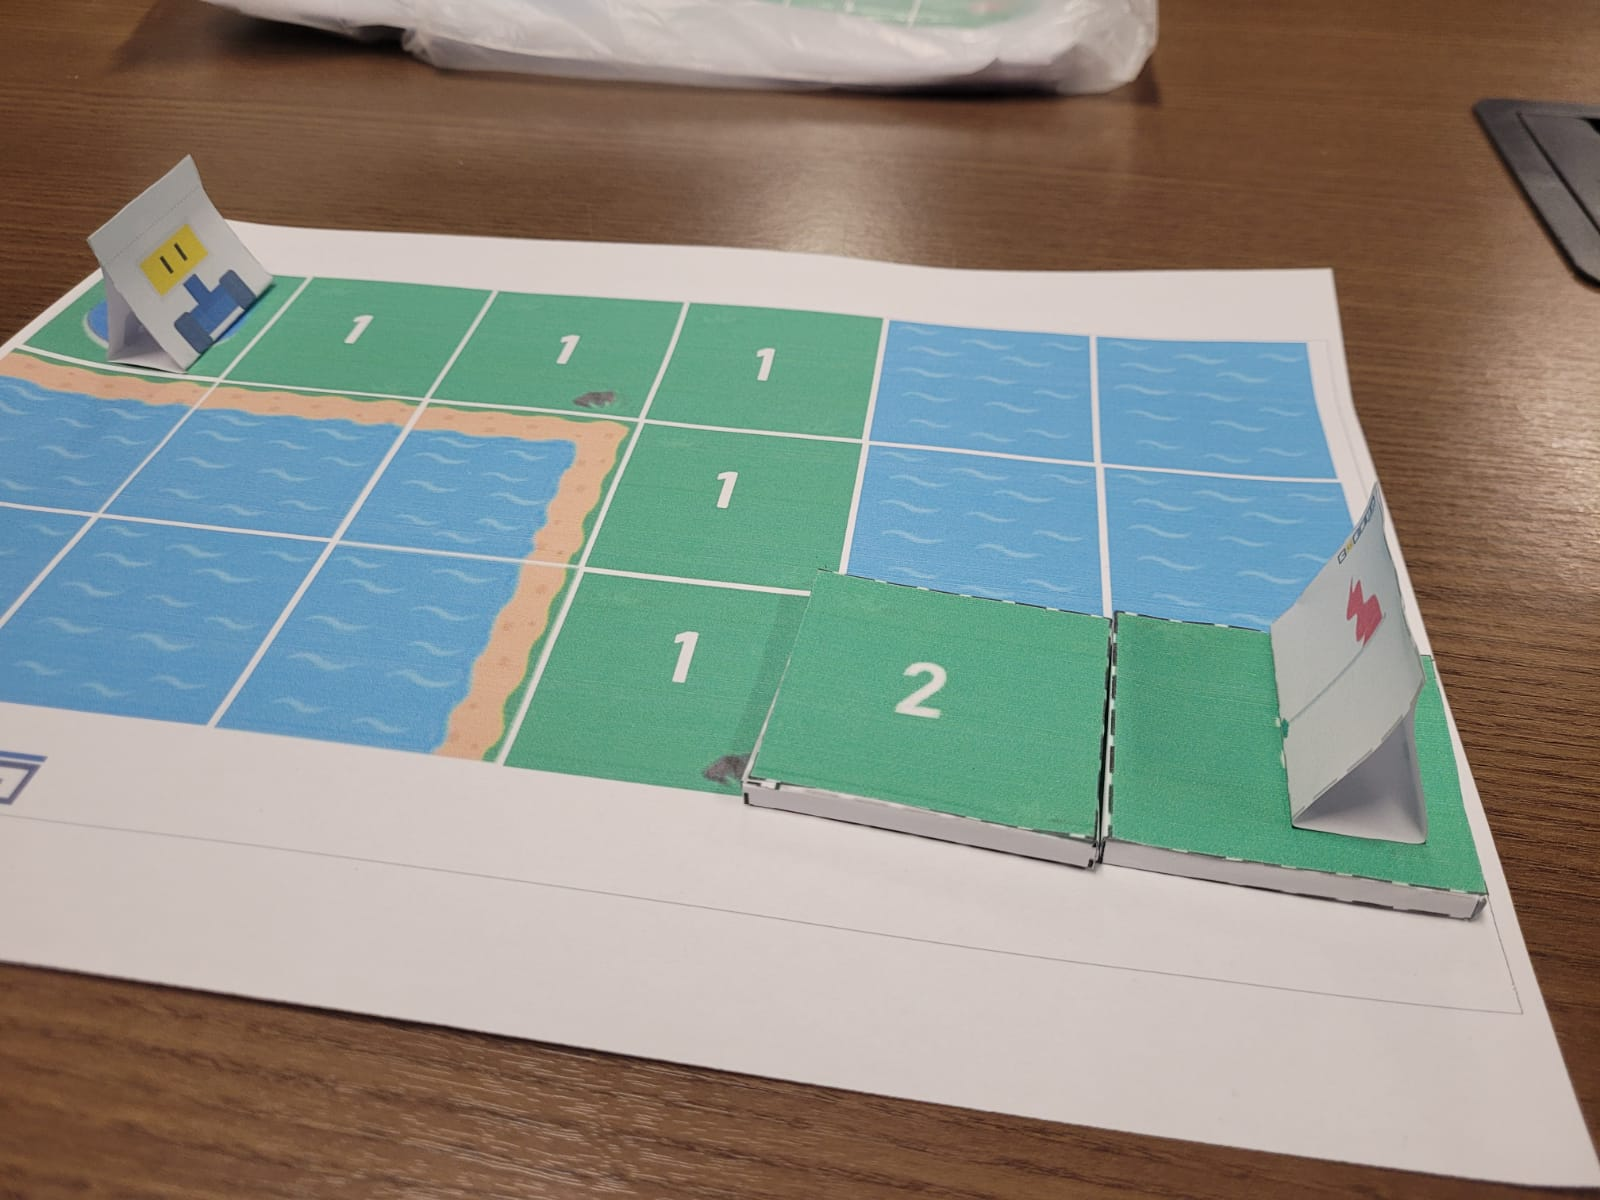
\includegraphics[width=0.8\textwidth]{images/code-unplugged.png}
	\legend{Fonte: \cite{de2023codebo}}
	\label{fig:codebo_unplugged}
\end{figure}


  \subsection{Desenvolvimento de um Jogo para Auxílio no Ensino de Estruturas de Dados}

Durante o trabalho de conclusão de curso intitulado \emph{"Desenvolvimento de um Jogo para Auxílio no Ensino de Estruturas de Dados"}, foi desenvolvido um jogo digital mobile com o intuito de facilitar e auxiliar o ensino, a aprendizagem e a visualização dos conceitos de algoritmos de busca da disciplina de Estrutura de Dados. A tecnologia utilizada para desenvolver este jogo foi a linguagem de programação Dart, em conjunto com o framework Flutter.

Por se tratar de um \emph{quiz}, a abordagem de ensino é explicita. \cite{glatz2023desenvolvimento}

\begin{figure}[H]
	\centering
	\caption{Captura de tela do jogo para auxiliar em estrutura de dados}
	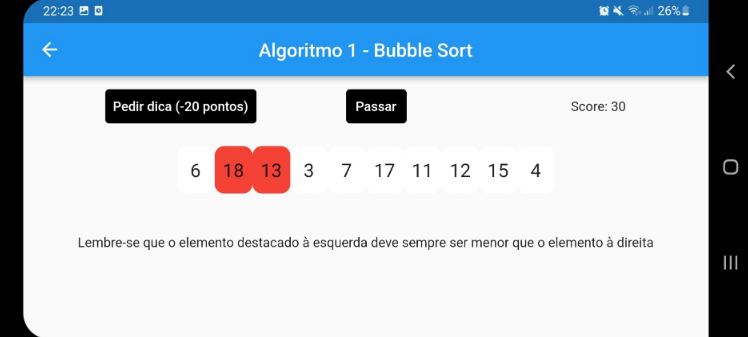
\includegraphics[width=0.8\textwidth]{images/aux-ed.png}
	\legend{Fonte: \cite{glatz2023desenvolvimento}}
	\label{fig:aux_ed}
\end{figure}


  \item \textbf{Prog-poly: Jogo de tabuleiro baseado no monopoly para ajudar nos estudos de linguagem de programação e engenharia de software}

Durante o trabalho de pesquisa de mestrado Prog-poly \cite{nascimento2022prog},
foi desenvolvido um jogo de tabuleiro com o intuito de facilitar e auxiliar a
aprendizagem de temas como linguagem de programação e engenharia de software.

Este jogo foi baseado na mecânica do clássico jogo de tabuleiro Monopoly, onde
cada jogador deve comprar propriedades no tabuleiro. Entretanto, este jogo se
diferencia pois para ter a oportunidade de comprar a propriedade, o jogador
deve responder de forma correta perguntas a respeito de ILPC (Introdução
Linguagem de Programação C) e, somente se acertar, poderá adquirir a
propriedade, caso possua dinheiro suficiente. Ganha o jogador que possuir a
maior quantidade de dinheiro e propriedades.

Este Jogo se caracteriza por ser um jogo com uma abordagem de ensino explicita, pois se trata de um \emph{quiz}. \cite{nascimento2022prog}

\begin{figure}[H]
	\centering
	\caption{Captura de tela do tabuleiro de Prog-poly}
	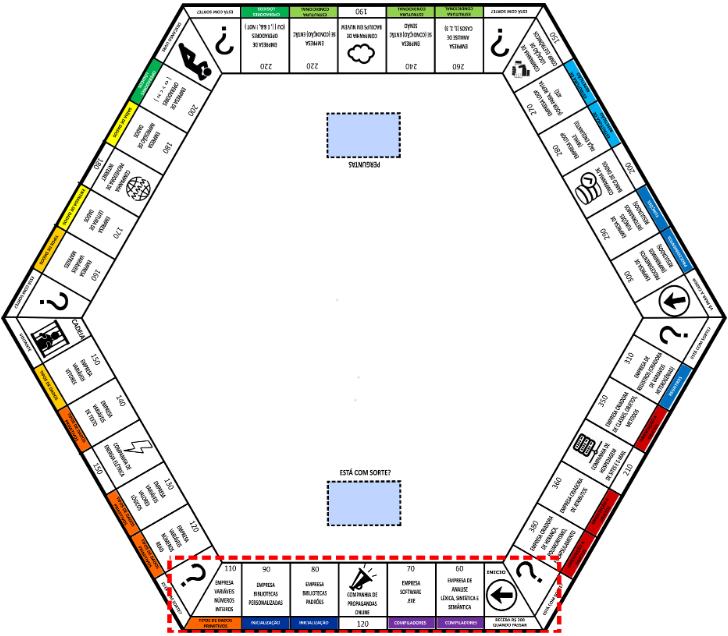
\includegraphics[width=0.8\textwidth]{images/prog-poly.png}
	\legend{Fonte: \cite{nascimento2022prog}}
	\label{fig:prog_poly}
\end{figure}


\end{enumerate}

 Por fim, foi efetuada uma comparação entre os trabalhos correlatos e este trabalho, demonstrada na \autoref{tab:cmp_trabalhos_relatos}.

\subsection{Comparação dos artigos}

Com base na análise dos cinco trabalhos selecionados, observa-se uma variedade
de abordagens no uso de jogos sérios para o ensino de conceitos de programação.
Cada proposta apresenta escolhas distintas quanto aos conceitos abordados,
estilo visual, mecânicas de interação e a forma como os conteúdos educacionais
são apresentados ao jogador.

A \autoref{tab:cmp_trabalhos_relatos} a seguir apresenta uma síntese
comparativa dos trabalhos analisados, destacando os aspectos centrais de cada
proposta e os elementos recorrentes identificados entre eles.

Os critérios utilizados para a comparação incluem:

\begin{itemize}
  \item \textbf{Jogo Digital (JD)} - Indica se o jogo é digital ou físico.
  \item \textbf{Conceitos de Estrutura de Dados (CED)} - Quais conceitos foram abordados:
    \begin{itemize}
      \item Pilha (P)
      \item Fila (F)
      \item Lista (L)
      \item Lista Encadeada (LE)
      \item Lista Duplamente Encadeada (LDE)
      \item Árvore Binária (AB)
      \item Algoritmo de Busca (B)
      \item Algoritmo de Ordenação (O)
    \end{itemize}
  \item \textbf{Forma de Abordagem Educacional (Ensino)} - Define se o ensino é tratado de forma explícita ou implícita.
  \item \textbf{Estilo} - Representação visual do jogo.
  \item \textbf{Gênero} - Categoria do jogo.
\end{itemize}

\begin{table}[H]
	\caption{Comparação entre os trabalhos relacionados}
	\label{tab:cmp_trabalhos_relatos}
	\centering
	\footnotesize
	\begin{tabular}{r|clllll}
		\toprule
		\textbf{Trabalho}      & \textbf{JD}  & \textbf{CED} & \textbf{Ensino}    & \textbf{Estilo}      & \textbf{Gênero}   \\
		\midrule
		Condigjob              & Sim          & -            & Explícito          & Simulador            & Puzzle            \\
		CodeBô                 & Sim          & F,L,P,B      & Implícito          & Isométrico           & Puzzle            \\
		CodeBo Unplugged       & Não          & P            & Implícito          & Tabuleiro            & Puzzle            \\
		AuxED                  & Sim          & B            & Explícito          & P\&C                 & Puzzle            \\
		Prog-poly              & Não          & -            & Explícito          & Tabuleiro            & Quiz              \\
		\bottomrule
	\end{tabular}
	\caption*{Fonte: Autor}
\end{table}


